%%
%  ******************************************************************************
%  * #file    Szablon_raportu_EN_Latex.tex
%  * #author  Adrian Wójcik   adrian.wojcik(at)put.poznan.pl
%  *          
%  * #commit  Patryk Kościk   koscikpatryk(at)gmail.com
%  *          Modified the template for Projekt przejsciowy purposes          
%  *          
%  * #version 1.0
%  * #date    09-Mar-2022
%  * #brief   PROJPRZEJ
%  *
%  ******************************************************************************
%%  
\documentclass[11pt, a4paper]{article}

\usepackage{SM_template}

% Wypełnijcie te dyrektywy zgodnie z waszym tematem
% \lab      -> NAZWA CZUJNIKA, np.: 'DHT22'
% \comment  -> Króciutki opis co to, np.: 'Cyfrowy budżetowy czujnik temperatury'
%
\lab{APDS-9960}
\comment{Czujnik RGB, oświetlenia i wykrywacz gestów \\ Szymon Kwiatkowski}

% Absolutny zakaz dotykania tego tutaj bo jak dotkiecie to coś jebnie
\university{Politechnika Poznańska}
\faculty{Wydział Automatyki, Robotyki i Elektrotechniki}
\institute{Instytut Robotyki i Inteligencji Maszynowej}
\department{Zakład Sterowania i Elektroniki Przemysłowej}
\addbibresource{bib/APDS-9960.bib}
\nocite{*}


%%
%
% Początek dokumentu
%
%%
\begin{document}

%% Strona tytułowa %%
\mainpage{{APDS-9960/APDS-9960.jpg}}
\newpage

\section*{Opis elementu} \addcontentsline{toc}{section}{Wstęp}
Moduł z czujnikiem, który mierzy natężenie światła otoczenia, umożliwia wykrywanie bliskości obiektu oraz wykrywa gesty dłoni. Przy pomocy tego sensora można kontrolować urządzenia poprzez machnięcie ręki. Układ pracuje z napięciem 3,3 V, komunikuje się poprzez I2C. Czujnik jest stosowany w Samsungu Galaxy S5. Układ pracuje z napięciem 3,3V. Czujnik jest w stanie rozróżnić następujące ruchy:
\begin{itemize}
    \item Prawo
    \item Lewo
    \item Góra
    \item Dół
    \item Opuszczanie ręki w kierunku czujnika
    \item Podnoszczenie ręki od czujnika
\end{itemize}
Schemat układu czujnika prezentuje się następująco:
\begin{figure}[H]
    \centering
    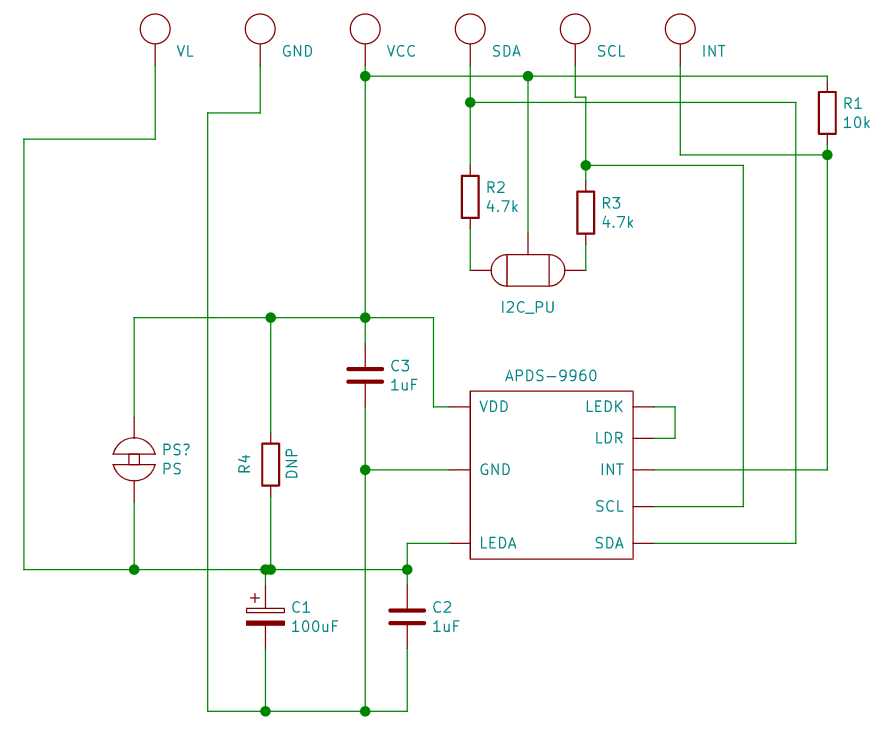
\includegraphics[width=0.7\textwidth]{fig/APDS-9960/polaczenie_modulu/schemat.png}
    \caption{Caption}
\end{figure}
Jak możemy zauważyć na schemacie układ posiada dwa pola które domyślnie nie są ze sobą zlutowane. Jednym z nich jest I2C PU natomiast drugim PS. I2C PU odpowiada za podciągnięcie układu pod dwa domyślnie rezystory podciągające dla magistrali I2C pod które układ ten nie jest podłączony domyślnie. Zworka PS służy z kolei do załączenia zasilania dla modułu diód podczerwonych znajdujących się również na plytce. Załączając tą funkcjonalność jesteśmy zmuszeni do podłączenia zasilania $VL$, które odpowiada za zasilanie tych komponentów.


\newpage

\section{Użycie czujnika}
Dane pochodzące z czujnika jesteśmy w stanie odebrać dobierając adres ramki jako 0x39. Po obraniu tego adresu jako domyślnego adresu z którego jesteśmy w stanie odebrać informacje możemy następnie odbierać je po linii I2C. Jednak by to zrobić warto zapoznać się z dokumentacją producenta znajdującej się w linku bibliografii ze strony forbot\cite{FORBOT}. Wszystkie parametry powinny zostać zainicjalizowane by uzyskać poprawne funkcjonowanie czujnika. Oprócz tego musimy uruchomić interfejs szeregowy I2C. Płytka domyślnie posiada możliwość podciągnięcia rezystorów pullup jeżeli tylko będziemy chcieli. Można to osiągnąć poprzez wcześniej przytoczoną zworkę I2C PU. Po spełnieniu tych kroków warto zorientować się odnośnie tego czy musimy zapewnić zasilanie dla ledów. Jeżeli zworka PS jest zlutowana to nie musimy podpiąć zasilania VL, jeżeli tak nie jest to jest taka konieczność. Następnie odczytujemy wartości kryjące się pod interesującym nas adresem i możemy zająć się ich obróbką. Same wartości najlepiej rozkodować zgodnie z dokumentacją producenta.

Zalecane przez producenta jest użycie paczki z biblioteką która umożliwia pracę z czujnikiem. Jest ona napisana do płytki arduino jednak wraz z oprogramowniem takim jak platformIO jesteśmy w stanie zbudować kod na STM32 jeżeli tylko przemapujemy odpowiednie piny. Warte odnotowania jest to że pobierając oprogramowanie należy uwzględnić zmiany w ID urządzenia APDS-9960 które różni się od tego sprzedawanego przez sparkfun. Dla nas będzie to id równe 0x39 które jest widoczne na odwrocie płytki HW-325.

\subsection{Proces pobierania informacji}
Jeżeli chcemy pobierać wstępnie wszystkie informacje z interfejsu I2C to koniecznym będzie:
\begin{itemize}
    \item Odpowiednie przypisanie wartości dla wszystkich rejestrów znajdujących się w dokumentacji
    \item Dla wybranego trybu pracy czujnika(Wykrywanie kolorów, gestów, kolorów i gestów), odpowiednia inicjalizaacja rejestrów
    \item Realizacja odczytu danych z czujnika:
    \begin{itemize}
        \item Wyczyszczenie wszystkich flag i statusów(interrupt line, fifo itp.)
        \item Zaadresowanie czujnika jego ID
        \item Pobór danych za pomocą ramki odnoszącej się do odpowiedniego rejestru
        \item Po poborze danych wyczyszczenie wszystkich kolejek oraz rejestrów dla interrupt
    \end{itemize}
\end{itemize}
Jeżeli chodzi o rejestry to są one dostępne w dokumentacji czujnik APDS-9960 która jest dostępna na stronie forbot\cite{FORBOT} oraz pliki z biblioteką oraz przykładami dla wyszczególnionych zadań czujnika znajdują się na stronie sparkfun\cite{PRZEWODNIK}.
\subsection{Implementacja i weryfikacja zadania czujnika}
Po wgraniu programu do płytki arduino bądź STM możemy za pomocą interfejsu szeregowego obserwować to jakie dane mamy wysyłane(Za pomoc Serial). Stan funkcjonowania czujnika można również zweryfikować po ciągłym zapalaniu i gaszeniu się czerwonej diody w jednym z czujników która jest uruchomiona za każdym razem kiedy dochodzi do zaadresowania i odczytu danych.

Przykładowe dane wyjściowe dla czujnika realizującego zadanie badania naświetlenia:
\begin{figure}[H]
    \centering
    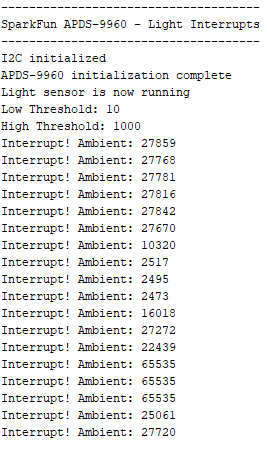
\includegraphics[width=0.5\textwidth]{fig/APDS-9960/zasada_dzialania/daneAmbient.png}
    \caption{Dane pojawiające się na porcie szeregowym dla przykładowego rozwiązania z przykładów na Arduino}
\end{figure}
Na zdjęciu przedstawiono przykładowe dane wyjściowe kolejno dla:
\begin{itemize}
    \item Naświetlenia w normalnym pokoju ze światłem dziennym
    \item Naświetlenia dla czujnika przesłoniętego palcem(duży spadek wartości ale nie całkowity do 0)
    \item Naświetlenia latarkę z telefonu(65535) - przekroczono maksymalny zasięg liczbowy
\end{itemize}
Ważne jest to że w trybie interrupt zasłaniąc czujnik obiektem nie emitującym niczego nie dochodzi do zajścia zdarzenia dla czujnika i tym samym nie wykonmy żadnego działania. Oznacza to że samoczynnie odbierzemy dane kiedy wykryjemy zbocze opadające na wejściu mikrokontrolera pochodzącymi z wyjścia INT czujnika.


\newpage
\printbibliography[heading=bibintoc]

\end{document}